\documentclass[12pt]{article}
\usepackage{amsmath}
\usepackage{setspace}
\usepackage{adjustbox}
\usepackage{graphicx}
\usepackage{float}
\usepackage{multicol}
\usepackage{hyperref}
\usepackage{subfig}
\usepackage{wrapfig}
\usepackage{xcolor}
\usepackage{tabularray}
\usepackage{sidecap}
%\usepackage{natbib,url}
\usepackage[backend=biber,style=numeric,maxnames =2,giveninits = true]{biblatex}
\addbibresource{journal_abbreviations.bib}
\addbibresource{References.bib}
\usepackage[margin = 1in]{geometry}
\usepackage{fancyhdr}
\usepackage{sectsty}
\usepackage{titlesec}


\sectionfont{\fontsize{14}{15}\selectfont}
\subsectionfont{\fontsize{12}{15}\selectfont}
%\bibliographystyle{abbrv}
\DeclareBibliographyDriver{std}{%
  \usebibmacro{bibindex}%
  \usebibmacro{begentry}%
  \usebibmacro{author/editor+others/translator+others}%
  \usebibmacro{title}%
  \setunit{\labelnamepunct}\newblock
  %\usebibmacro{title}%
    %\newunit\newblock
  \usebibmacro{journal}
  \newunit\newblock
  \usebibmacro{date}%
  \newunit\newblock
\usebibmacro{finentry}}

\DeclareBibliographyDriver{stdbook}{%
  \usebibmacro{bibindex}%
  \usebibmacro{begentry}%
  \usebibmacro{author/editor+others/translator+others}%
  \setunit{\labelnamepunct}\newblock
  %\usebibmacro{title}%
  \usebibmacro{title}
  \newunit\newblock
  \usebibmacro{date}%
  \newunit\newblock
\usebibmacro{finentry}}

%\DeclareBibliographyAlias{article}{std}
%\DeclareBibliographyAlias{book}{stdbook}
%\DeclareBibliographyAlias{misc}{stdbook}
\AtEveryBibitem{% Clean up the bibtex rather than editing it
 \clearfield{isbn}
 \clearfield{doi}
 \clearfield{url}
 \clearfield{issn}
 }
\AtBeginBibliography{\small}
\definecolor{gray_c}{rgb}{0.745, 0.898, 0.898}
\definecolor{gray_h}{rgb}{0.43, 0.72, 0.72}

%\titlespacing\section{0pt}{12pt plus 4pt minus 2pt}{0pt plus 2pt minus 2pt}
\titlespacing\subsection{0pt}{12pt plus 4pt minus 2pt}{0pt plus 2pt minus 2pt}
%\titlespacing\subsubsection{0pt}{12pt plus 4pt minus 2pt}{0pt plus 2pt minus 2pt}

\def\epo{\epsilon\rightarrow 0}
\def\lb{\left(}
\def\rb{\right)}
\def\ls{\left[ \vphantom]}
\def\rs{\right] }
\def\ep{\epsilon}

\title{Direct simulation of ocean-ice coupling in icy moons}
\author{Tobias Oliver}
\date{}

\begin{document}
\pagestyle{fancy}
\thispagestyle{fancy}
%... then configure it.
\fancyhf{} % clear all header fields
\fancyhead[L]{\textcolor{red}{Tobias Oliver\\
Research Proposal}}
\fancyfoot[R]{\thepage}
\newcommand{\citep}[1]{\cite{#1}}
\begin{center}
\large{\textbf{Dynamic ocean-ice coupling on icy moons}}
\end{center}

I propose to study the effects of salinity on convective processes in the icy moons of our Solar System and beyond. 
I will investigate the interplay of horizontal and bottom driven convection, and the competing effects of temperature and salinity via a novel suite of tailored numerical simulations. 
I will focus on the interaction between the subsurface oceans and the overlaying ice in order to understand their coupled dynamics. 
%\textbf{With upcoming data from the \textit{Europa Clipper} and \textit{JUICE} missions, the results from this study can be used to relate surface observations to ocean dynamics}.
\textbf{The proposed work is relevant to a broad range of planetary bodies, but it will particularly serve the \textit{Europa Clipper} and \textit{JUICE} space missions by providing insight for relating upcoming data to underlying ocean dynamics and its coupling with the ice crust}.

\section{Background}
The Solar System contains a number of icy bodies, many of which are thought to be ``ocean worlds'' and may be suitable candidates for the habitability of life \citep{tB24}.
Figure \ref{f:pic}(a) illustrates a proposed structure of these bodies. 
The Jovian satellites Europa, Callisto, and Ganymede, as well as the Saturnian moon Enceladus, were all identified as likely ocean worlds after data returned from the \textit{Galileo} and \textit{Cassini} missions \citep{fN16}.
The sub-surface oceans link the solid cores of these moons to their icy exteriors. Circulations within the oceans govern the transport of heat and chemicals to the icy surface \citep{kS20}. 

%It is likely that these oceans are turbulent and capable of convecting heat and chemicals between the solid interior and icy crust
%.
%A variety of forcing mechanisms have been proposed and discussed, such as electromagnetic coupling\citep{cGlP19}, tides, and precession\citep{kS24}, and in this investigation 
These oceans are believed to be extremely turbulent, and multiple mechanisms for driving circulation have been proposed \citep{kS24}.
%Multiple mechanisms are proposed to drive circulations in these ocean, which are believed to be extremely turbulent \cite{kS24}.
%The circulations in these oceans are driven by multiple mechanisms, and are believed to be extremely turbulent \citep{kS24}.
I propose to study buoyancy driven flows, in which variations in the fluid density drive convection.
I will consider the contributions of temperature and salinity to density variations.
%ensity variations are due to heterogeneities in both temperature and salinity.
%Heterogeneities in both temperature and salinity contribute to density variations.
%Density variations are usually attributed to two separate mechanisms-- heterogeneities in temperature and salinity. The associate density variations drives convection and references \citep{yA21,wK22} predict that this mechanism serves to flatten the ice shell of Europa (ie.  homogenous thickness).

%\begin{wrapfigure}{R}{0.6\textwidth}
%\end{wrapfigure}
\begin{figure}[H]
	\begin{center}
		\subfloat[][]{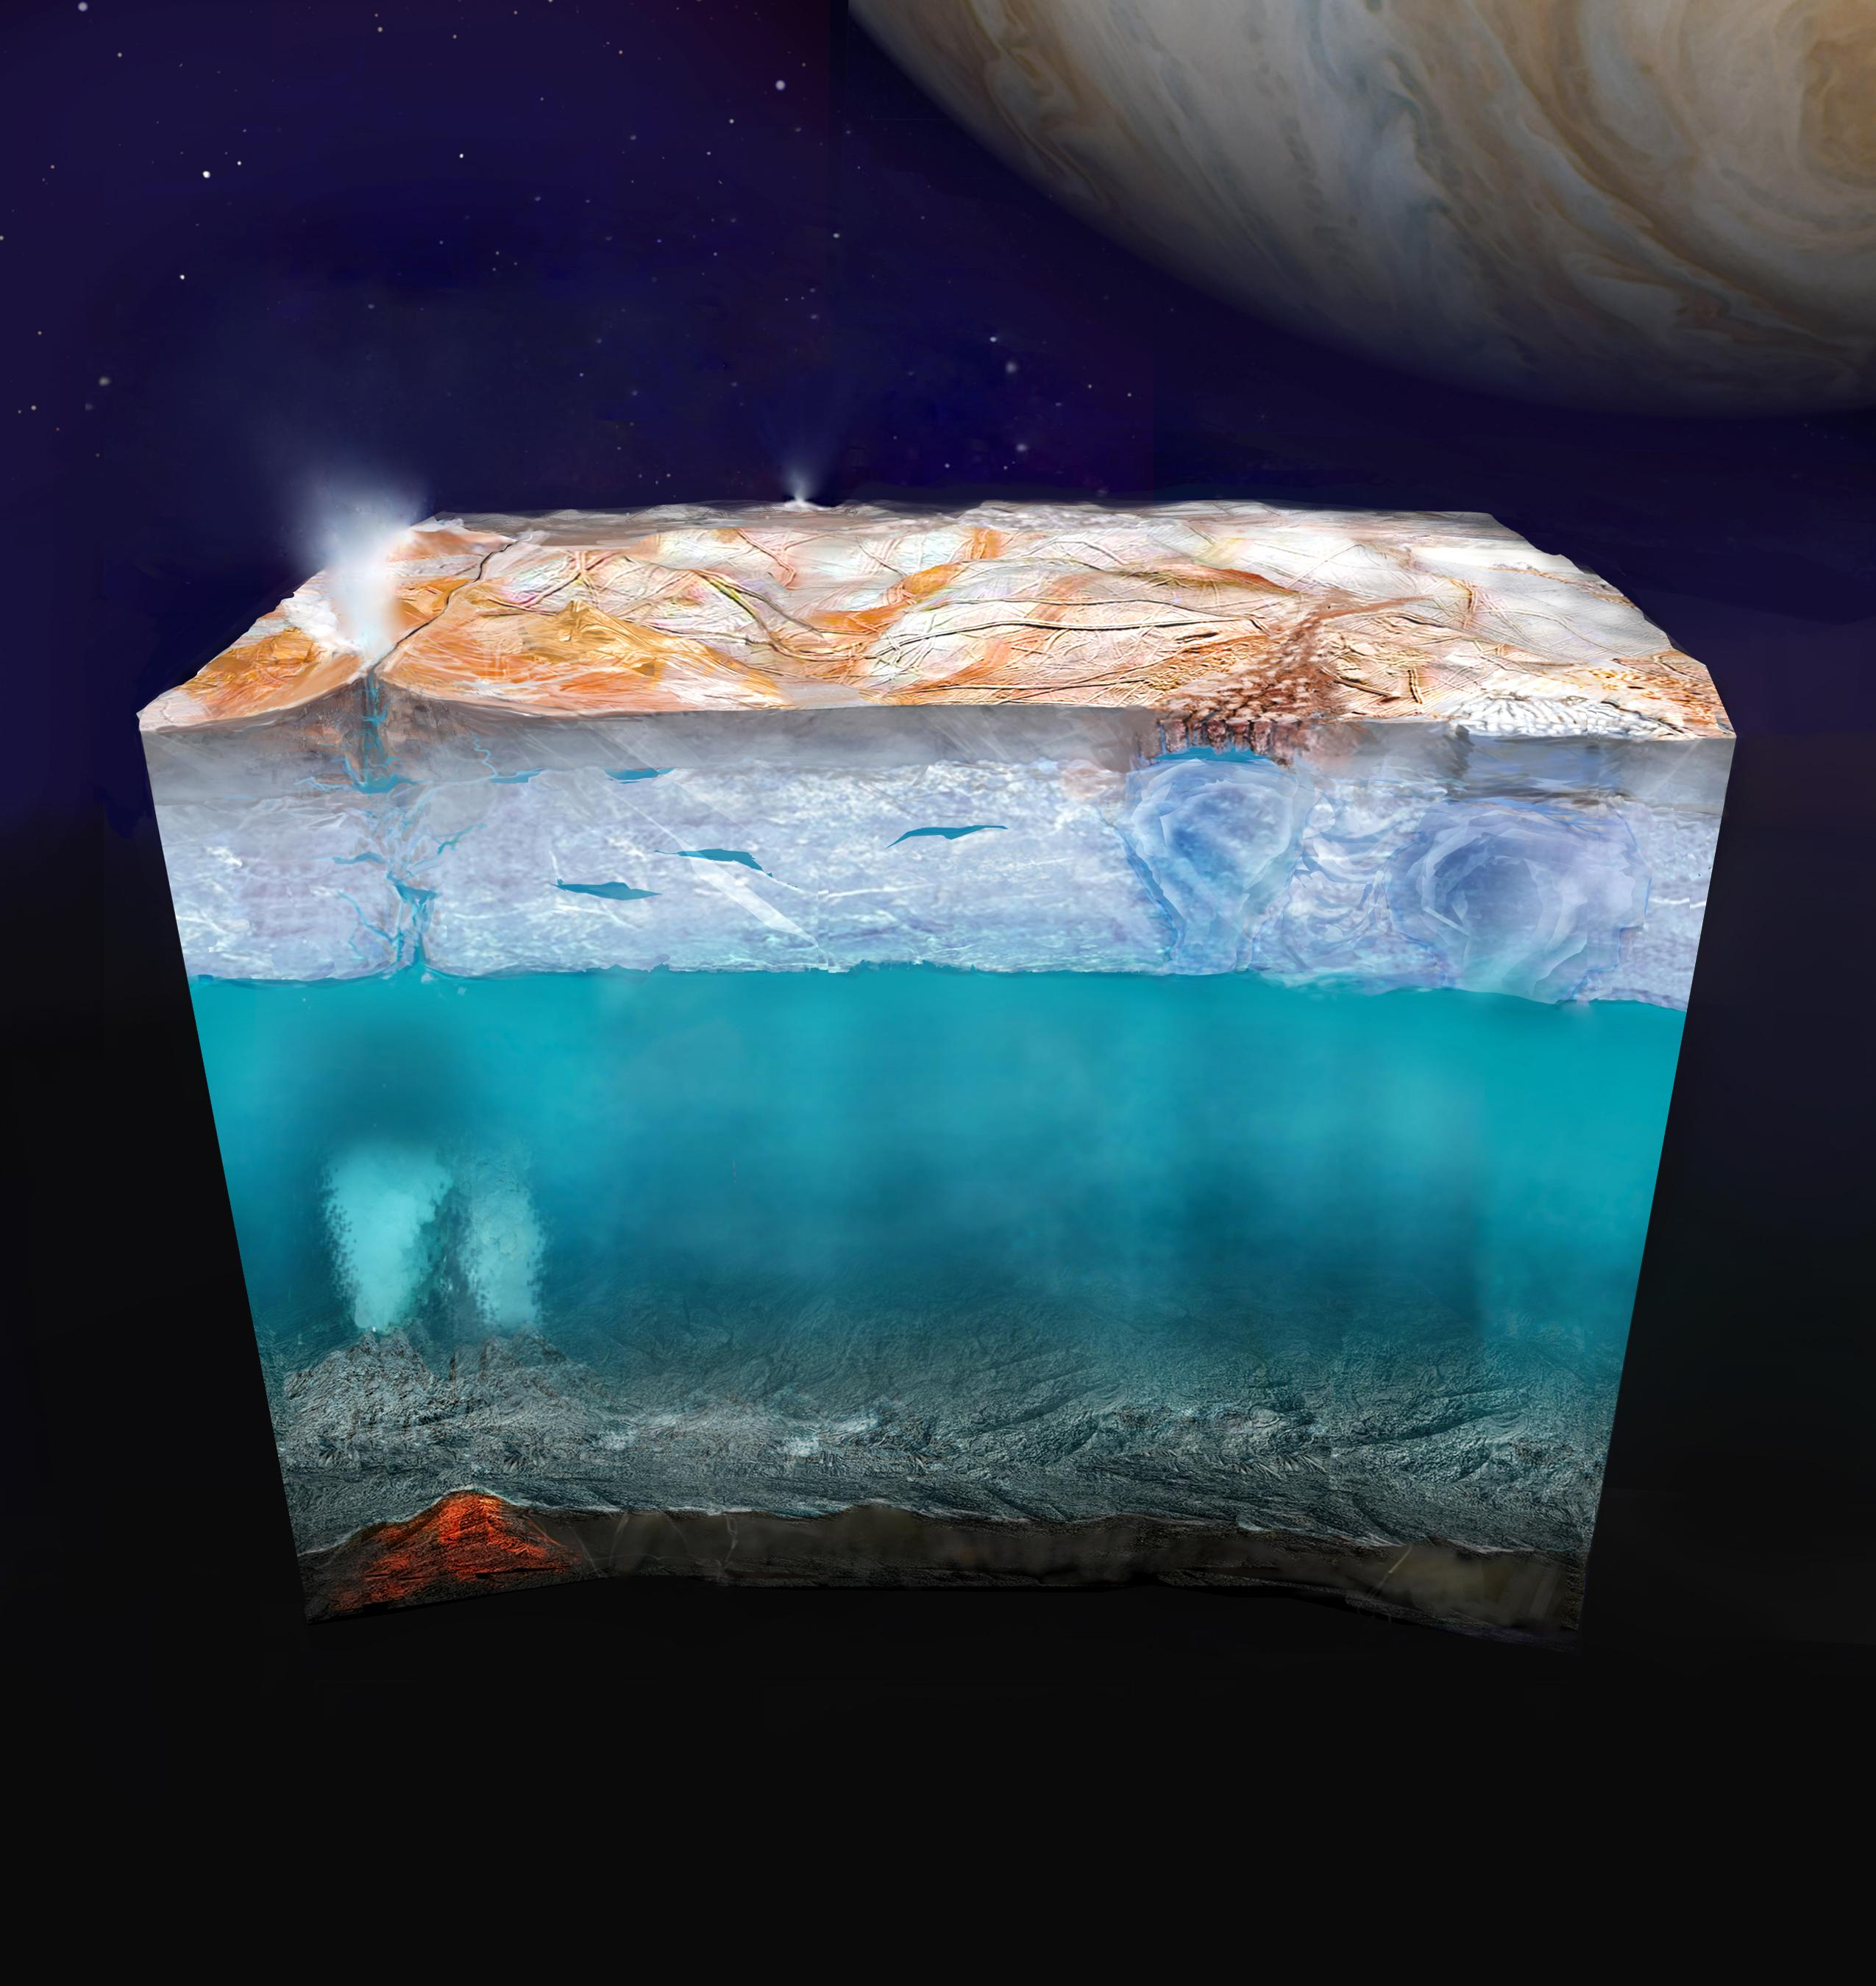
\includegraphics[width=0.25\textwidth]{figures/europa_ice}}
		\quad
		\subfloat[][]{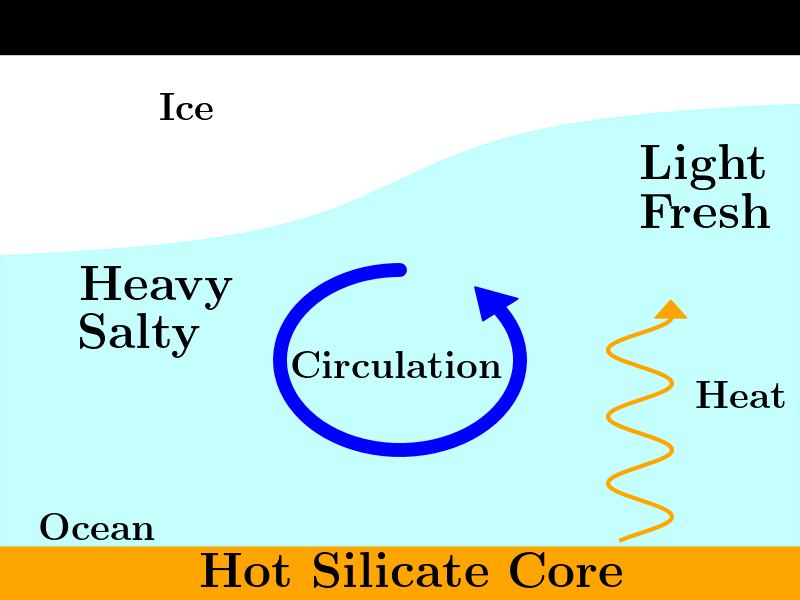
\includegraphics[width=0.35\textwidth]{figures/hc}}
	\subfloat[][]{\includegraphics[width=0.25\textwidth]{figures/conv}}
	\end{center}
	\caption{(a) Artist interpretation of subsurface ocean on Europa, not to scale (NASA/JPL-Caltech). (b) Possible mechanism for horizontal convection driven by heterogeneous melting. Adapted from \citep{wK22}. Snapshot of temperature from a simulation (by PI) of thermal bottom driven convection in a planetary core \citep{tO25}.}
	\label{f:pic}
\end{figure}

Two different mechanisms for convection will be considered.
Horizontal convection (HC) results from density heterogeneities on the icy surface. Heavy fluid sinks and light fluid flows in to replace it, as illustrated in figure \ref{f:pic}(b). This drives a circulation within the ocean. Bottom driven convection (BDC) is due to density differences between the fluid near the silicate core and the fluid at the icy surface. Lighter fluid near the core rises while heavier surface fluid sinks, once again setting up a circulation. 
%In plane layers, BDC is often referred to as Rayleigh-B\'enard convection. 
It is proposed that BDC is driven by radiogenic heating from the silicate core \citep{kS14,kS19,jK22}. A snapshot of a simulation of BDC in a planetary interior from the PI's dissertation is shown in figure \ref{f:pic}(c) \citep{tO25}. 
\textbf{In a rotating planet, heat fluxes due to BDC will vary with latitude \citep{kS14}. This indicates lateral variations in melt, which are expected to drive HC \citep{wK22}.}
The competition and interplay between these two mechanisms in spherical geometry, including the effects of rotation and salinity, is the purpose of the proposed project.


\section{Proposed project and methodology}

\textbf{In this project I propose to study the interaction between melt on the icy shell with the underlying convecting ocean via numerical simulations of a coupled ice-ocean system.} This will be the first study to consider thermal and saline convection in a full spherical geometry.
I will focus on the heat flux through the icy shell, and use these results to make predictions about temperature distributions and melt on the icy moons. These predictions will directly serve the upcoming the \textit{Europa Clipper} and \textit{JUICE} missions.

There are two major technical challenges associated with this study. The first is that it is not possible to perform fluid simulations in the actual parameter regimes of the icy moons. The second is generating a consistent model for heat fluxes into the ice and the resulting melt and release of fresh water.
In the following two sections, I outline my approach to handle these difficulties.
\subsection{Key nondimensional parameters}
In convection studies, we solve dynamical equations governing the conservation of energy, momentum, and salinity. However, there is a large disparity between the scales relevant to planetary bodies and the scales that can be simulated. 
Usually this issue is formalized in terms of nondimensional numbers that represent the ratios of different physical effects in the system. %Alterntively, we can think of these quantities as ratios of different forcing terms in the governing equations. 
%In a geophysical and astrophysical context, there are two non-dimensional numbers of particular importance: the Rayleigh and Ekman numbers. 
The Rayleigh number $Ra$ describes the ratio of buoyancy to diffusivity. In planetary interiors, $Ra$ is very large, generally indicating vigorous convective turbulence.
The Ekman number $Ek$ is the ratio of viscous diffusion to Coriolis effects. Values for $Ek$ tend to be very small, indicating that rotation plays an important role.
For salty oceans, a buoyancy ratio $\Gamma$ quantifies the relative effects of temperature and salinity on density.
%Two other quantities of importance are the Nusselt number, $Nu$, and Prandtl number, $Pr$. 
%They are the ratio of total heat transfer to conductive heat transfer and the ratio of momentum to thermal diffusivity respectively \citep{kS19}. 
Explicitly, these parameters are
\[Ra = \frac{g\alpha\Delta T D^{3}}{\nu\kappa_{T}},\quad Ek = \frac{\nu}{\Omega D^{2}},\quad \Gamma = \frac{\alpha\Delta T}{\beta \Delta S}\]% \quad Nu = \frac{hD}{k_{O}} \quad Pr= \frac{\nu}{\kappa_{T}},\]
where $g$ is the surface gravitational acceleration, $\alpha$ and $\beta$ are the coefficient of thermal and saline expansion respectively, $D$ is the ocean thickness, $\nu$ and $\kappa_T$ are the diffusivities of momentum and temperature respectively, and $\Omega$ is the planetary rotation rate.
%, $h$ is the total heat transfer, and $k_O$ is the thermal conductivity of the ocean. 
$\Delta T$ is the temperature difference between the ocean surface and floor. $\Delta S$ is the average ocean salinity. 
The ratio of the ocean thickness to the moon radius will be fixed to $0.1,$ which is icy-moon like and identical to previous studies \citep{dL23,kS19}.

The Biot number, \textit{Bi}, is the ratio of conductive resistance to convective heat flow \citep{jL24}. A large value of $Bi$, relevant to icy moons, indicates that convective processes are important to determine the ice-ocean temperature response.
In our simulations $Bi$ is an output value, but we can control it by varying $D_{i}$, the thickness of the ice layer. 

%A compositional Rayleigh number $Ra_{S}$ can be defined by replacing $\alpha, \Delta T,\text{ and, }\kappa_{T}$ with the associated quantities for salinity.

To take Europa as an example, predicted values of $Ra$,  $Ek$, and $Bi$ are $O\lb 10^{20}\rb $, $O\lb 10^{-12}\rb $, and $O\lb 10^{6}\rb $ respectively \citep{dL23}. $\Gamma$ is poorly constrained but estimates suggest it is much less than unity \citep{yA21}. In the context of icy moons, numerical simulations have only reached values of $Ra \le 10^{9}$ and $Ek \ge 10^{-6}$ \citep{dL23}. 
%In studies of different planetary bodies, more aggressive simulations have been performed (eg. figure \ref{f:pic}(b), references \citep{tO25}), however all fall significantly short of reaching realistic values. For icy moons, it is particularly difficult to reach small values of $Ek$ because the ocean depth is much smaller than the planetary radius. 
\textbf{The procedure is to establish scaling laws with the nondimensional parameters by simulating at moderate values, and then extrapolating to planetary values}. 
%$Bi$ can be varied by simulating at different values of $D_{i}$. 
Prior work \citep{yA21} considered thermal and saline convection, but only for single values of $Ra$ and $Ek$, which prohibits extrapolation to extreme values.

The parameter space that I will explore is provided in table \ref{t:param}. Overlap with previous studies \citep{dL23,kS19} is intended, as it will allow me to compare my findings with these ``purely thermal" results. This will better elucidate the added effects of saline convection.
%I will explore similar parameters to the regimes studied in references \citep{dL23,kS19}. This will allow me to best compare these ``purely thermal'' results to my findings, which will better elucidate the new effects of saline convection. 
I will sweep across an order of magnitude in $\Gamma$ to establish a scaling relationship with the buoyancy ratio. 
%A complete list of the proposed simulations is given in table \ref{t:param}. 
\subsection{A dynamically coupled ice-ocean model}

Horizontal convection is driven by salinity variations at the outer boundary of the liquid domain. In order to investigate this mechanism, it is necessary to couple the heat fluxes into the ice with melt into the ocean. 
Convective studies that do not consider salinity have generally only investigated the ocean \citep{kS19,dL23} and not the ice. The general approach is to fix the temperature of the bounding surface (ice shell), however this implies uniform melt.
\textbf{I propose to use a simulation configuration in which the ice is included in the solution domain so that heat is able to conduct from the ocean into the ice.} 
A boundary condition for temperature is placed on the moon surface, and the temperature of the ocean-ice interface is allowed to vary. The interfacial temperature can be used to determine the salinity at the ocean surface \citep{wK22}.
\textbf{This approach has never been used in a full spherical geometry.}


\begin{table}
\begin{center}
\begin{tabular}{|c|c|c|c|c|c|}
\hline
$Ra$&$Ek$&$D_{i}/D$& $\Gamma$ &\# Simulations & Cost (cpu$\times$hour)\\
		\hline
$\lb 5 \times 10^{6} - 2 \times 10^{8} \rb $ & $3 \times 10^{-4} $ & $0.5,0.1$&0.5,0.05&20&$1.7 \times 10^{6}$\\
  	\hline
$\lb 5 \times 10^{6} - 1 \times 10^{9} \rb $ & $1 \times 10^{-4} $ & $0.5,0.1$&0.5,0.05&20&$1.7\times 10^{6}$\\
  	\hline
$\lb 5\times 10^{7}, 2 \times 10^{9} \rb $ & $3 \times 10^{-5} $ & $0.5,0.1$&0.5,0.05&8&$2.5\times 10^6$\\
		\hline
%Shell & $10^5$& $\infty$&$10^4-10^5$& 5& $2\times 10^{6}$\\
%		\hline
%Shell & $10^5$& $10^{-4}$&$10^4-10^5$& 5& $2\times 10^{6}$\\
%		\hline
%Plane &$5\times10^{5}-2\times10^{6}$ & $3\times10^{-4}$&$12.5Ra$ &5 &$2.5\times 10^{5}$  \\
%		\hline
%Plane &$10^{6}-10^{7}$ & $10^{-4}$&$12.5Ra$& 5 & $5\times 10^{5}$\\
%		\hline
%Plane &$10^{7}-5\times 10^{7}$ & $3\times10^{-5}$&$12.5Ra$ & 5& $10^{6}$ \\
		\hline
Totals & & & &48&$4.9 \times 10^6$ \\
		\hline
\end{tabular}
\end{center}
\caption{Proposed parameter space. The third column presents the ratio of ice to ocean thickness, which can be modified to change $Bi$. Computing costs are estimate values based off of existing studies \citep{dL23,rM19} and personal experience with relevant codes.}
\label{t:param}
\end{table}


\subsection{Proposed simulations and computing requirements}
I propose a suite of 48 simulations to investigate ice-ocean coupling in the icy moons. The specific parameter values are given in table \ref{t:param}, as well as the estimated computing cost.  The existing hydrodynamics code \texttt{Nek5000} \citep{nek5000} will be used to perform the simulations, and can be configured to handle thermal-saline convection as well as the solid icy exterior.
Simulations will be performed in spherical shells to best represent the icy moon geometry.
Table \ref{t:param} provides estimate computing times based on previous rotating convection studies in icy moons \citep{dL23} and my experience with \texttt{Nek5000}.
 I will apply for computing time through ACCESS and the Texas Advanced Computing Center, which both provide access to high performance computing resources and have supported me in the past. The host institutions also provide computing time.
 \subsection{Timeline}
 I estimate that constructing the code and model will take one year. This will include building and testing a simplified planar model which can be used to gauge the feasibility of the proposed parameter regime. Planar models are generally much cheaper to simulate and are useful for validating basic principles. If the proposed parameters are determined to be too extreme for the available computing time, then the most expensive simulations (low $Ek$) will be relegated to the cheaper planar model. Codes and methods to analyze the output will be developed during this time. The second year will be dedicated to performing the simulations in table \ref{t:param} and investigating the differences between pure BDC and coupled BDC and HC. In the third year I will focus on developing predictions that can be tested by \textit{Europa Clipper} and \textit{JUICE} based on my results.%\begin{figure}

\section{Scientific motivation}
\subsection{The Jovian system and beyond}
The primary objective of NASA's \textit{Europa Clipper} (EC)\cite{pC14_EC} and ESA's \textit{JUICE} \citep{oG13} missions is to investigate Europa, Ganymede, and Callisto, three Jovian satellites believed to be ocean worlds. Each is expected to contain salty, liquid oceans underneath thin icy shells \citep{rP99,fN16}, and both EC and \textit{JUICE} aim to determine whether these bodies contain necessary conditions for life \citep{tB24}. 

The dynamics of these oceans are poorly understood, and neither mission will be able to make direct observations of the oceans, however multiple observations are planned that will hint at the ocean dynamics. For example, EC will use radar altimetry to determine surface topography and a magnetometer to constrain salinity profiles with depth \citep{jR23}.  
A deeper understanding of the interaction between the convection and icy surface is necessary, and is outlined as one of the key future issues in the recent review of icy moon oceanography \citep{kS24}.


The proposed study will investigate the thermal response of the icy shell to the underlying convection, and the ocean's response to the melting and freezing shell. 
%\textbf{When data from EC and \textit{JUICE} becomes available, these results will provide insight into the interior of the Jovian ocean worlds.}
\textbf{These results will provide insight into the interior of the Jovian ocean worlds, which will be crucial to interpret the upcoming data from EC and \textit{JUICE}.}
%\subsection{Beyond the Jovian system}

This project applies to other planetary bodies as well. The Saturnian moon Enceladus likely contains a sub-surface ocean and has a similar geometry to Europa \citep{kS24}. There is significant uncertainty whether Triton \citep{jK22} and Pluto \citep{kS24} are ocean worlds and the results of this study will be useful to further constrain the properties of these bodies. 
Significantly less is known about exoplanets, although we may be able to extend our results in this regard as well.

Lastly, the studied convective processes have implications for induced magnetic fields and planetary dynamos. Our results will be useful in investigating the magnetic properties of planetary bodies in the Solar System and beyond.
%
\subsection{Long term goals}
The focus of my research has been convection in planetary interiors similar to the Earth's core, but I would like to increase my research perspectives to include other planetary bodies and terrestrial oceans. The icy moons are a crossroads between planetary convection and oceanography and present an exciting natural laboratory for studying rotating convection where new data is upcoming. This project would broaden my expertise and improve my outlooks when applying for research positions in the planetary sciences.

\begin{spacing}{0.4}
%\begin{multicols}{2}
%\bibliography{References,journal_abbreviations}%jfm-bib,References}

\printbibliography

%\end{multicols}
\end{spacing}
\end{document}
